\chapter{Rádiová komunikace}
Rádiová komunikace je druhou nejdůležitější funkcí LG vesty. Využívá se k nakonfigurování vest před hrou, a během hry k předávání informací mezi jednotlivými vestami a řídícím počítačem.

\section{Topologie sítě}
\begin{figure}[H]
    \begin{center}
        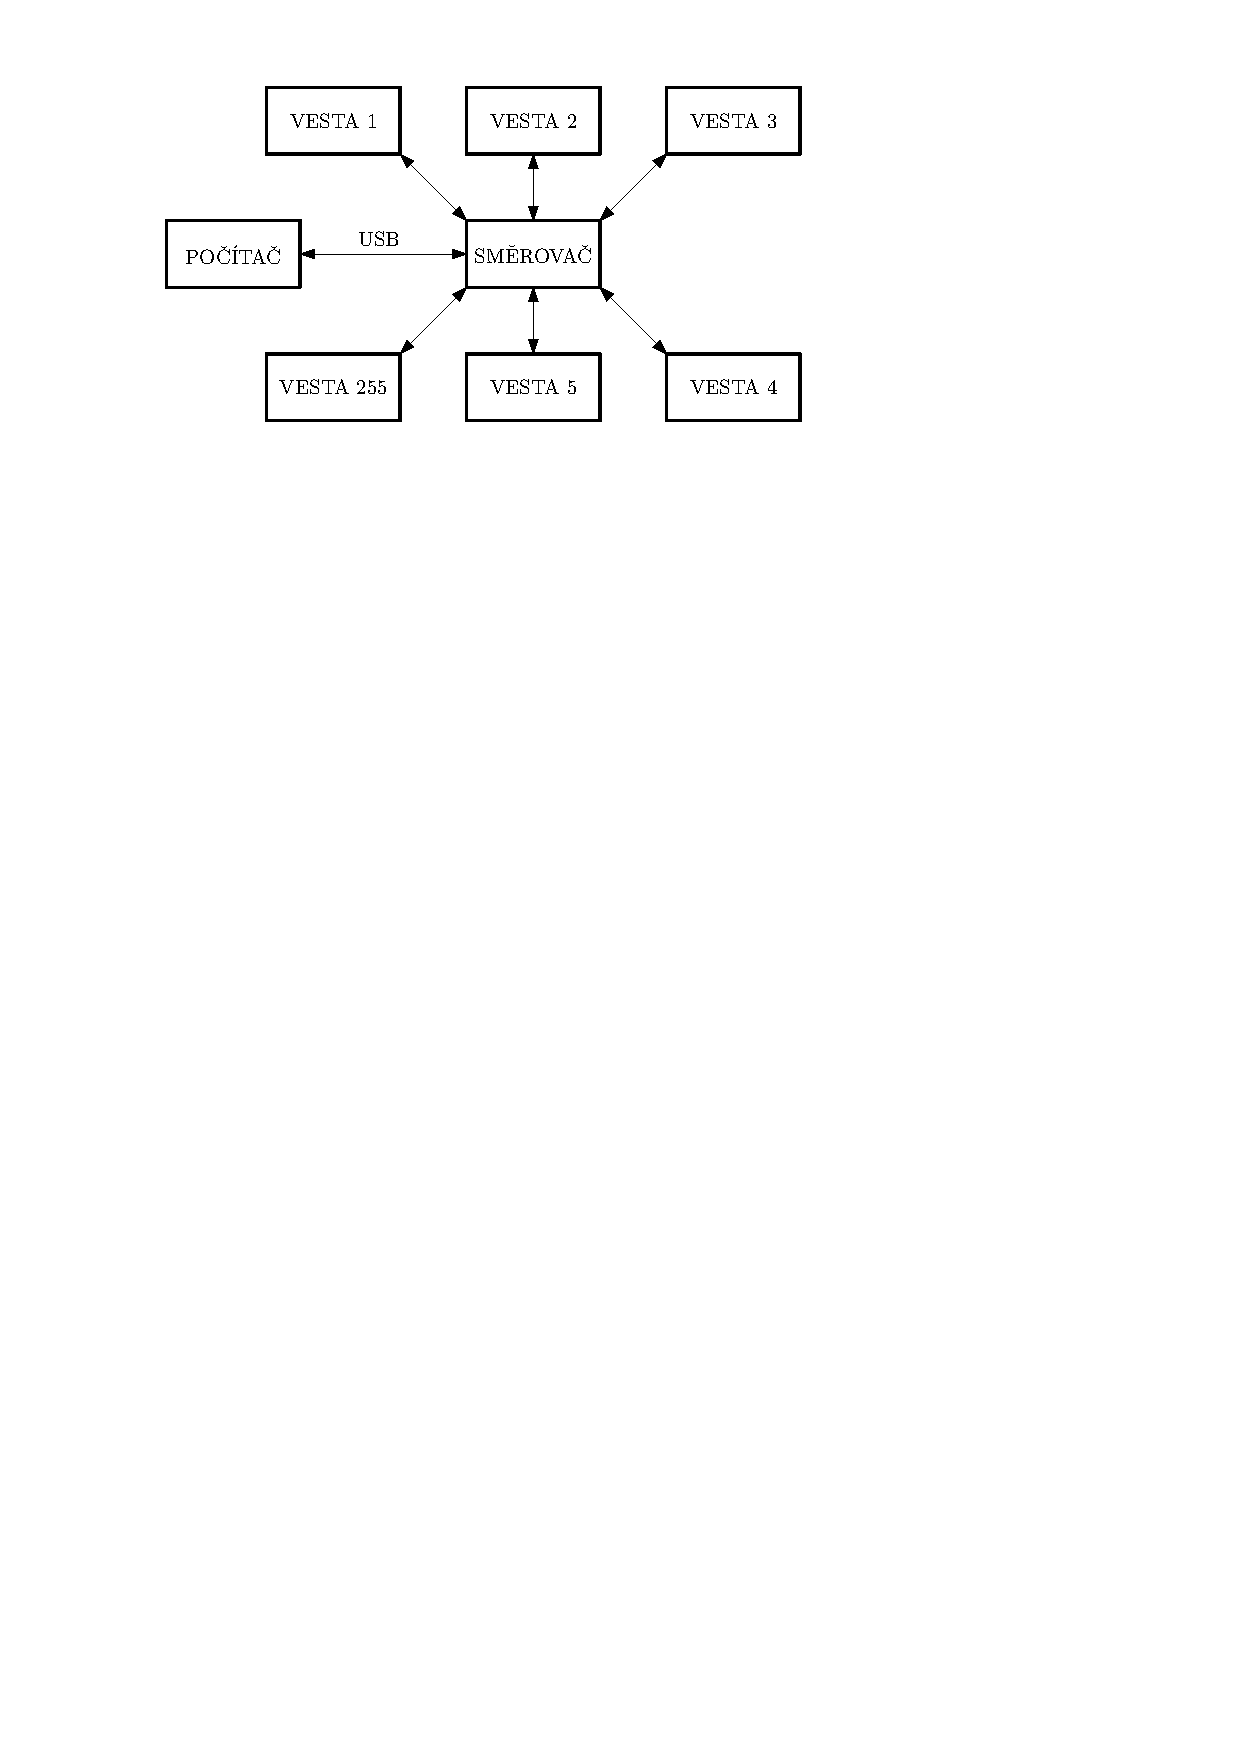
\includegraphics[width=0.7\textwidth]{img/rf-network}
    \end{center}
    \caption{blokové schéma topologie sítě}
\end{figure}
Byla použita hvězdicová topologie sítě, v jejímž středu se nachází router, který zprostředkovává komunikaci mezi řídícím počítačem na jedné straně a vestami na straně druhé. Tato topologie je výhodná, protože nedochází ke konfliktům mezi jednotlivými zařízeními. Router uděluje jednotlivým zařízením v síti časová okna, kdy mohou komunikovat. Router je tedy v této síti v roli řídícího prvku a ostatní zařízení jsou pouze řízená.

\section{Přenášený rámec}
\begin{figure}[H]
    \begin{center}
        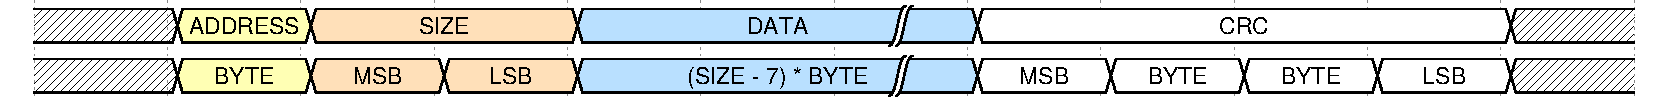
\includegraphics[width=\textwidth]{img/lgrf_packet}
    \end{center}
    \caption{znázornění rámce rádiové komunikace}
\end{figure}

Přenášený rámec má proměnnou délku v závislosti na velikosti přenášených dat, jelikož je třeba přenášet data o velikosti pár bytů při zjišťování stavů vest, tak i data o velikosti stovek bytů při konfigurování zařízení. Pro kompletní konfiguraci vesty však zcela postačuje velikost 512~\jedn{B}.

Rámec začíná 8~\jedn{b} adresou, která specifikuje příjemce, resp. odesílatele. Následují dva bajty udávající počet bytů v rámci. Poté jsou v rámci umístěna přenášená data. Rámec končí čtyřmi bajty obsahujícími 32~\jedn{b} CRC, které slouží jednak k potvrzení správnosti přenášených dat a také k vyhledávání platných rámců v přijatých datech.

\section{Praktická realizace}
\begin{figure}[H]
    \begin{center}
        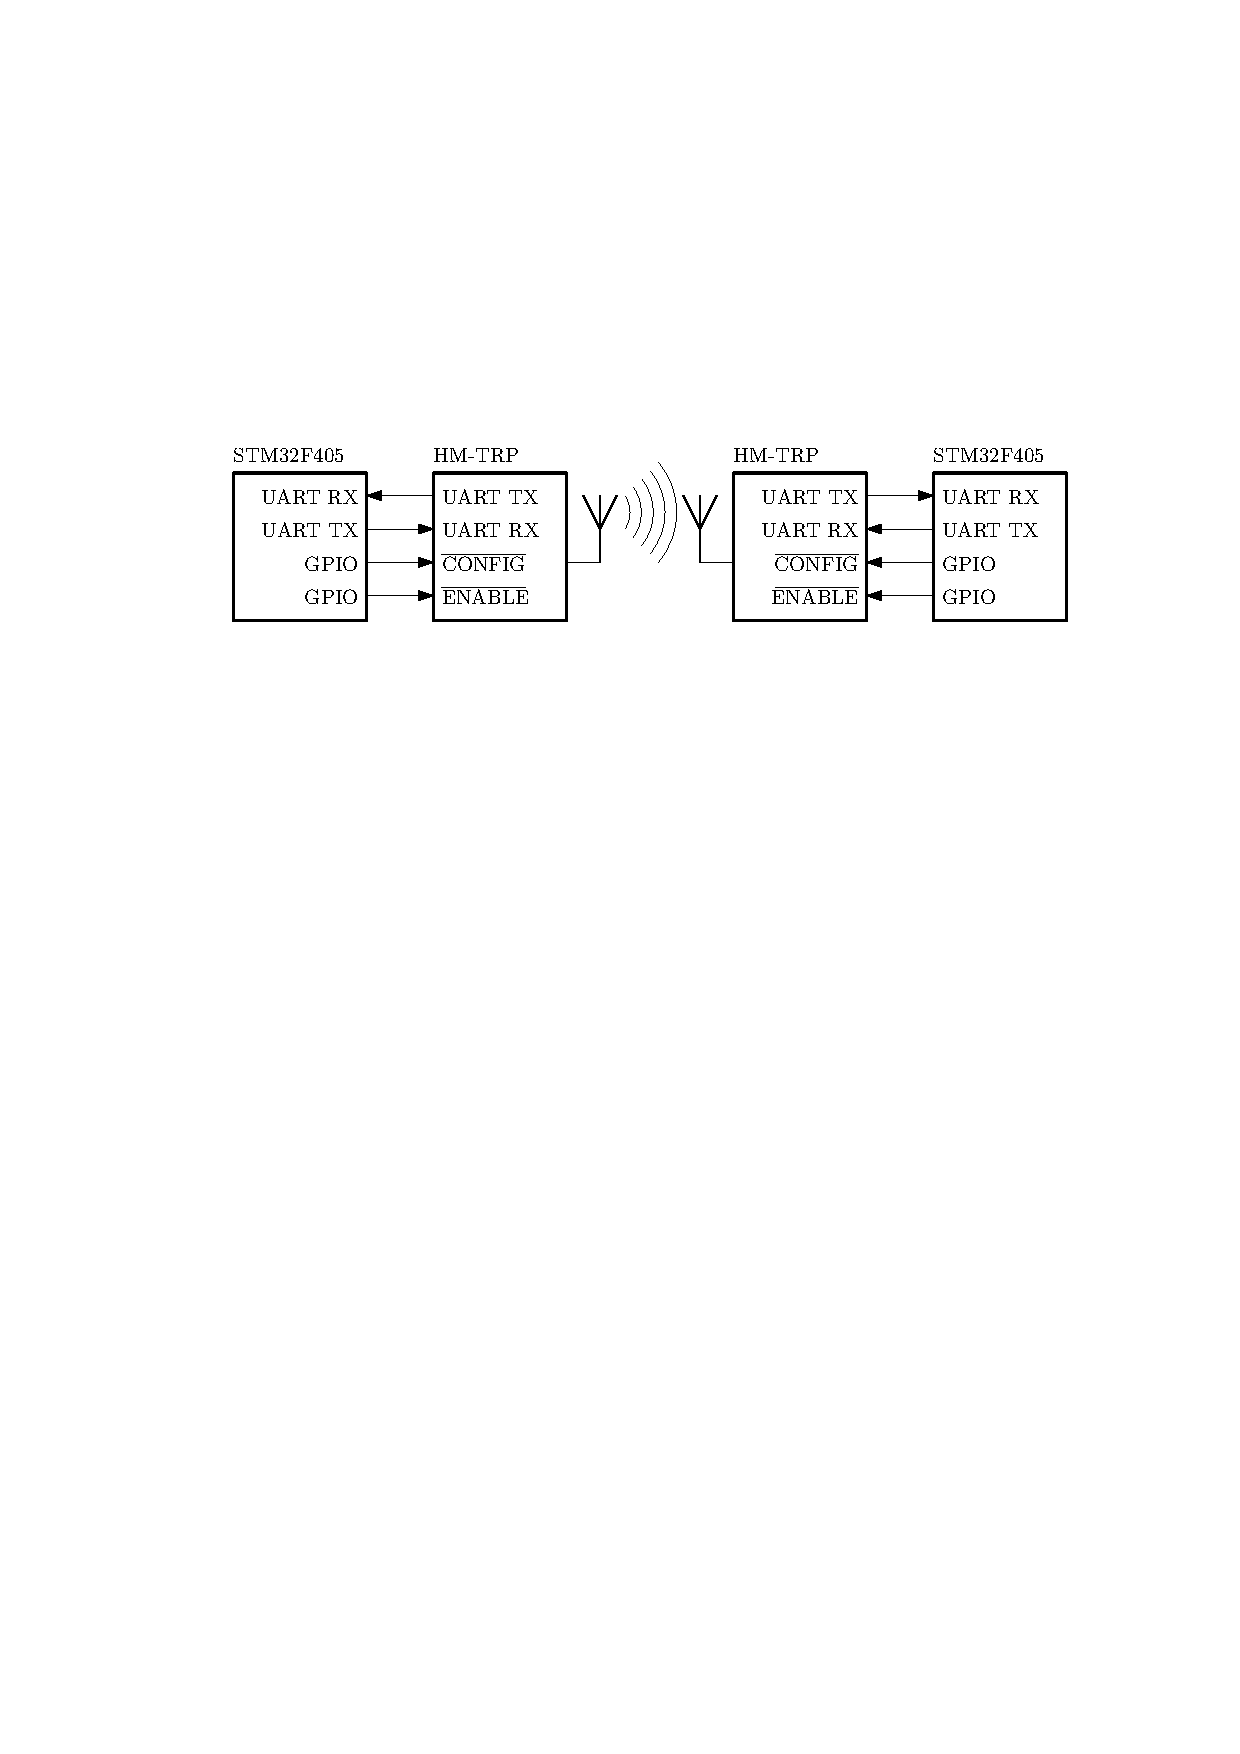
\includegraphics[width=\textwidth]{img/hm-trp}
    \end{center}
    \caption{blokové schéma jednoduchého komunikačního řetězce z moduly HM-TRP}
\end{figure}
Rádiové rozhraní je postavené na modulech HM-TRP firmy Hope Microelectronics. Moduly mají programovatelnou pracovní frekvenci, systém používá 868~\jedn{MHz}. Dále mají nastavitelný vysílací výkon $\in \langle 1; 20 \rangle~\jedn{dBm}$. Moduly pracují v poloduplexním módu, tedy v jeden okamžik mohou buďto přijímat nebo vysílat. Dále jsou moduly vybaveny rozhraním UART, umožnujícím snadnou komunikaci z modulem (přijímat a vysílat přenášená data a také modul konfigurovat). Moduly poskytují pouze možnost vysílat a přijímat data, která jsou do něj pomocí UART poslána, avšak negarantují úspěšnost doručení dat na místo určení. Tento problém je třeba řešit n vyšší vrstě komunikace.
